\clearpage

\lehead[]{\sf\hspace*{-2.00cm}\textcolor{white}{\colorbox{lightblue}{\parbox[c][0.70cm][b]{1.60cm}{
\makebox[1.60cm][r]{\thechapter}\\ \makebox[1.60cm][r]{ÜBUNG}}}}\hspace{0.17cm}\textcolor{lightblue}{\chaptertitle}}
\rohead[]{\textcolor{lightblue}{\chaptertitle}\sf\hspace*{0.17cm}\textcolor{white}{\colorbox{lightblue}{\parbox[c][0.70cm][b]{1.60cm}{\thechapter\\
ÜBUNG}}}\hspace{-2.00cm}}
%\chead[]{}
\rehead[]{\textcolor{lightblue}{AvHG, Inf, My}}
\lohead[]{\textcolor{lightblue}{AvHG, Inf, My}}

\section{Übungsaufgaben: Client/Server}

\subsection{Aufgabe 1: Einfacher Client}

Im Kurs-Repository findest du die ausführbare JAR-Datei
\myFile{SimpleServer.jar}. Wenn du diese startest, läuft der Server auf Port
\lstinline|11111|. Schreibe einen Client, der eine Verbindung zu diesem Server
herstellt. Der Benutzer sollte die Bezeichnung des Servers in einem Textfeld
eingeben können. Die Portnummer kann fest in das Programm eingebaut werden. Der
Server sendet an den Client einen kurzen Text und beendet dann die Verbindung.
Das Client-Programm soll den Text in einem Textfeld ausgeben.

\begin{center}
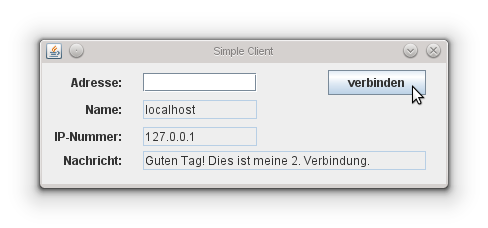
\includegraphics[width=0.6\textwidth]{./inf/SEKII/43_Java_ClientServer/SimpleClient.png}
\end{center}

\subsection{Aufgabe 2: Echo-Client}

Im Kurs-Repository findest du die ausführbare JAR-Datei
\myFile{EchoServer.jar}. Wenn du diese startest, läuft der Server auf Port
\lstinline|22222|. Der Echo-Server sendet alle Daten, die an ihn geschickt
werden, wieder an den Absender zurück. Schreibe einen Client, der eine
Verbindung zum Echo-Server aufbaut. Der Benutzer kann den Namen des Servers
eingeben. Nachdem die Verbindung erfolgreich aufgebaut wurde, kann der Benutzer
in einem Textfeld Sätze eintippen. Sobald er auf den daneben stehenden Button
drückt, wird die eingegebene Zeile an den Server gesendet. Wenn eine Verbindung
aufgebaut wird, wird für das Einlesen der Daten, die der Server zurücksendet,
ein eigener Thread erzeugt. Dieser Lese-Thread schreibt die empfangenen Daten
in eine \myClass{JTextArea} (eingebettet in eine \myClass{JScrollPane}) des
Anwendungsfensters. Die Verbindung zum Echo-Server kann über
einen Button getrennt werden. Wenn der Client die Verbindung beendet, schließt
auch der Server die Verbindung. Der Lese-Thread erhält nach dem Schließen der
Verbindung durch den Server eine \myClass{IOException}. Wenn er eine
\myClass{IOException} erhält, soll sich der Lese-Thread selbständig beenden.
Dies überprüft man am besten durch eine Ausgabe auf der Konsole.

\begin{center}
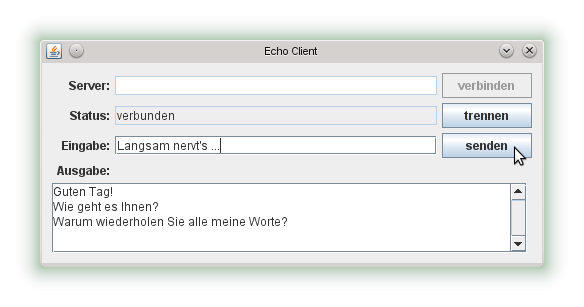
\includegraphics[width=0.75\textwidth]{./inf/SEKII/43_Java_ClientServer/EchoClient.png}
\end{center}

\subsubsection{Tipp: Zeilenumbrüche:}

Wenn man in der \myClass{JTextArea} eine neue Zeile anfangen möchte, kann man
dies kodieren, indem man nacheinander die Zeichen \emph{Carriage Return}
(Wagenrücklauf, ASCII-Zeichen Nr.\ 13) und \emph{Line Feed} (Zeilenvorschub,
ASCII-Zeichen Nr.\ 10) sendet. Man kann entweder die ASCII-Zeichen als
Integer-Werte senden oder sie mit Hilfe einer Escape-Sequenz in einem String
kodieren. Beispiel für die Kodierung eines Zeilenumbruchs in einem String:

\begin{lstlisting}
String text = "Erste Zeile\r\nZweite Zeile.";
\end{lstlisting}

\lstinline|\r| steht für Carriage Return

\lstinline|\n| steht für Line Feed

Sinnvoll ist, dass der EchoClient beim Senden eines Strings an den Server
automatisch einen Zeilenumbruch an den Text des Benutzer anfügt.

\textbf{Allerdings werden Zeilenumbrüche je nach verwendetem Betriebssystem
unterschiedlich kodiert (\lstinline|\\r\\n| ist richtig für Windows).
Sinnvoller ist es deshalb die statische Methode
\lstinline|System.lineSeparator()| zu benutzen. Sie erzeugt je nach verwendetem
Betriebssystem die richtige Zeichenfolge}:

\begin{lstlisting}
String text = "Erste Zeile" + System.lineSeparator() + "Zweite Zeile.";
\end{lstlisting}


\subsection{Aufgabe 3: HTTP-Client}

Das Herunterladen einer Web-Seite mit Hilfe des HTTP-Protokolls ist relativ
einfach. Web-Server benutzen laut Konvention immer den TCP-Port \lstinline|80|.
Nachdem ein Browser eine Verbindung zu einem HTTP-Server aufgebaut hat, kann er
mit folgendem Befehl eine Seite herunterladen:

\begin{lstlisting}
GET <Seite> <Protokoll>
\end{lstlisting}

Wenn man zum Beispiel die URL 

\url{http://www.heise.de/index.html}

laden möchte, baut man zuerst eine Verbindung zum Server mit dem Namen
\lstinline|www.heise.de| auf. Anschließend sendet man an den Server den Befehl:

\begin{lstlisting}
GET /index.html HTTP/1.0\r\n\r\n
\end{lstlisting}

Am Ende des Befehls müssen zwei Carriage Return/Line Feed Anweisungen gesendet
werden. Die dadurch gesendete Leerzeile am Ende bedeutet, dass keine weiteren
Informationen gesendet werden.

Der Server überträgt zuerst einen \glqq Header\grqq\ mit Zusatzinformationen wie
beispielsweise den Servertyp und das Datum der letzten Änderung und
anschließend den Inhalt der angeforderten Datei. Nach der Übertragung beendet
der Server die Verbindung. Der Browser muss den übertragenen HTML-Code
interpretieren und dem Benutzer geeignet anzeigen. Befinden sich in der Seite
Verweise auf Images, Applets oder Frames, so fordert der Browser die
entsprechenden Inhalte in weiteren \lstinline|GET|-Transaktionen vom Server an.

\subsubsection{Aufgabe}

Programmiere einen einfachen Mini-Browser, der eine Verbindung zu einem
HTTP-Server im Internet aufbauen kann und eine vom Benutzer angegebene Seite
anfordert. Die vom Server übertragenen Daten sollen in eine \myClass{JTextArea}
geschrieben werden.

Damit die Verbindung während der Übertragung der Daten gegebenenfalls beendet
werden kann, sollte das Lesen der Daten in einem eigenen Thread erfolgen, weil
das Frame sonst während des Einlesens nicht auf Tastendrücke reagieren kann. In
einer ersten, einfachen Test-Version kann man jedoch auf einen
Hintergrund-Thread verzichten und die Daten direkt in der
Ereignis-Behandlungs-Methode des Buttons (\lstinline|actionPerformed()|)
einlesen.

\begin{center}
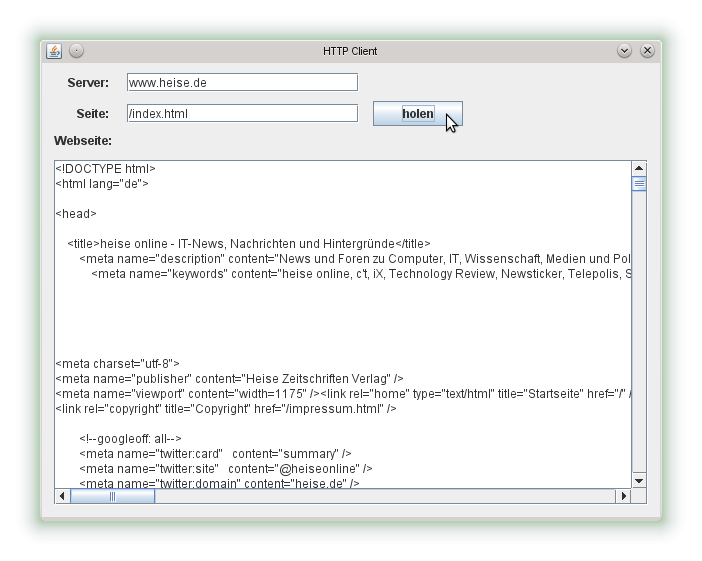
\includegraphics[width=0.89\textwidth]{./inf/SEKII/43_Java_ClientServer/HttpClient.png}
\end{center}

Tipp: Alternativ lässt sich mit wenig Zusatzaufwand die HTML-Seite auch richtig
darstellen:

\begin{center}
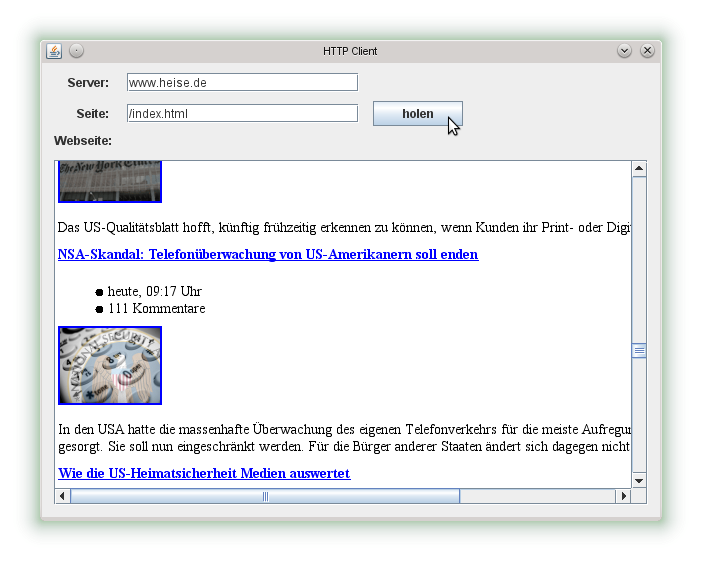
\includegraphics[width=0.89\textwidth]{./inf/SEKII/43_Java_ClientServer/HttpClient_HTMLEditorKit.png}
\end{center}

Dazu muss man lediglich die \myClass{JTextArea} durch eine \myClass{JTextPane}
ersetzen. Dann kann man wie folgt vorgehen:

\begin{lstlisting}
textPaneAusgabe = new JTextPane();
textPaneAusgabe.setEditorKit(new javax.swing.text.html.HTMLEditorKit());
\end{lstlisting}

Im Lese-Thread sammelt man dann zunächst alles, was vom HTTP-Server zurück
geliefert wird, ein und speichert es in einer String Variablen ab.

Zum Schluss wird das Ergebnis dann in der \myClass{JTextPane}-Komponente
dargestellt:

\begin{lstlisting}
int zeichen;
String html = "";
while ((zeichen = in.read()) != -1) {
    html += (char) zeichen;
}
main.textPaneAusgabe.setText(html);
\end{lstlisting}


\subsection{Aufgabe 4: POP3-Protokoll}

Startet das Programm \myFile{GenericClient.jar} aus dem Kurs-Repository.

Arbeitsaufträge:

\begin{compactenum}
\item Überprüft zunächst ob dieser Client sich gegenüber dem SimpleServer (Port
\lstinline|11111|) und dem EchoServer (Port \lstinline|22222|) genau so verhält
wie die zuvor von euch selbst programmierten Clients.

\item Mit dem im Standard RFC 1939 beschriebene Post Office Protocol 3 (POP3)
kann man e-Mails aus einem Postfach beim Provider abholen. POP3 benutzt den
TCP-Port \lstinline|110|.

\begin{compactenum}[a)]
\item Sucht im Internet nach Informationen zum POP3-Protokoll. Ihr braucht für
die weitere Arbeit eine Übersicht über die gängigsten POP3-Befehle.
\item  Überlegt und diskutiert untereinander, ob und wie man unseren Client dazu
verwenden könnte um e-Mails von einem POP3-Server abzuholen.
\end{compactenum}
 
\item Zum Testen könnt ihr den Server \lstinline|pop.1und1.de| benutzen.
Versucht die Mails des Benutzers\linebreak 
\myUserInput{AvHG@online.de} abzuholen.
Als Passwort gebt ihr \myUserInput{Humboldt} an.

\item Ihr könnt auch versuchen vorhandene e-Mails zu löschen. Wenn dies
erfolgreich war, solltet ihr an \myUserInput{AvHG@online.de} eine
e-Mail schicken, damit das Postfach wieder gefüllt ist.

\item Überlegt und diskutiert, ob mit diesem Client beliebige
Netzwerkserver (erfolgreich) kontaktiert und bedient werden können. Welche
Protokolle könnten wir noch testen?
\end{compactenum}


\subsection{Aufgabe 5: Einfacher Server}

Schreibe einen einfachen Server als Gegenstück zu dem einfachen Client, den wir
als erstes programmiert haben. Der Server besitzt ein Textfeld mit einer
Statuszeile, in der der aktuelle Zustand des Servers und die bisherige Anzahl
der Verbindungen angezeigt wird (siehe Abbildung). Um die korrekte Arbeitsweise
des Servers zu kontrollieren empfiehlt es sich, zusätzlich Debug-Ausgaben in
die Konsole zu schreiben (zum Beispiel \myUserInput{Verbindung aufgebaut},
\myUserInput{Verbindung beendet}).

\begin{center}
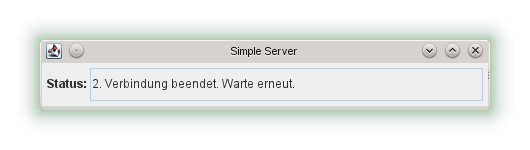
\includegraphics[width=0.6\textwidth]{./inf/SEKII/43_Java_ClientServer/SimpleServer.png}
\end{center}

Da der Haupt-Thread des Frames immer auf verschiedene Ereignisse (wie zum
Beispiel das Neuzeichnen des Fensters) reagieren muss, darf der Server nicht im
Thread des Frames auf ankommende Verbindungen warten, denn damit würde er die
Ereignisbehandlung blockieren. Es muss also ein zusätzlicher Thread generiert
werden, in dem der Server ankommende Verbindungen entgegen nimmt. Wenn eine
Verbindung aufgebaut ist, schickt der Server einen kurzen Text an den Client.
Damit jedes Mal ein anderer Text generiert wird, wird in dem Text die aktuelle
Verbindungsnummer eingebaut (zum Beispiel \myUserInput{Dies ist meine 10.
Verbindung.}). Nach dem Senden des Textes beendet der Server die Verbindung zum
Client und wartet mit \lstinline|accept()| auf die nächste Verbindung. Dieser
einfache Server braucht noch nicht mehrere Clients parallel bedienen zu können,
da die Dauer einer Verbindung äußerst kurz ist.


\subsection{Aufgabe 6: Echo-Server}

Programmiere einen Echo-Server, der alle Eingaben, die er von einem Client
erhält, wieder an den Client zurück sendet. Der Echo-Server soll mehrere
Clients parallel bedienen können. Wenn eine Client-Verbindung aufgebaut wurde,
generiert er für die Kommunikation mit dem Client einen eigenen Thread. Im
Konstruktor des Threads wird der Socket, der für diesen Client erzeugt wurde,
als Parameter übergeben. Der Thread beendet sich, wenn die Verbindung von
Seiten des Clients geschlossen wurde. Dies kann entweder durch eine Exception
angezeigt werden oder dadurch, dass der Server in der \lstinline|read()|-Methode
ein Byte mit dem Wert \lstinline|-1| erhält.


\subsection{Zusatzaufgabe: Chat-Client und -Server}

\subsubsection{Client}

Der Benutzer des Chat-Clients kann die Adresse des Servers und einen selbst
gewählten Namen eingeben. Nachdem der Benutzer einen Button gedrückt hat, baut
der Chat-Client eine Verbindung zum Chat-Server auf.

Der Benutzer kann über ein Textfeld zeilenweise Text eingeben, der an den
Server gesendet wird und vom Server an alle anderen angemeldeten Clients weiter
geleitet wird. Der Client sendet zuerst den selbstgewählten Namen des Benutzers
(damit die anderen Benutzer wissen, wer den Text gesendet hat), dann folgen ein
oder mehrere Trennungszeichen und dahinter der vom Benutzer geschriebene Text,
der mit einem Zeilenumbruch (\lstinline|System.lineSeparator()|) endet:

\lstinline|Name: Text|

Im Frame gibt es neben dem Eingabefeld eine \myClass{JTextArea}, in der alle
gesendeten Texte angezeigt werden. Das Empfangen der Texte vom Server geschieht
in einem Hintergrund-Thread. Die Texte können unverändert in die
\myClass{JTextArea} eingetragen werden. Die durch den Aufruf von
\lstinline|System.lineSeparator()| erzeugten Steuerzeichen sorgen dafür, dass
nach jedem Text ein Zeilenumbruch erfolgt.

\subsubsection{Server}

Der Server ermöglicht es einer beliebigen Anzahl Clients miteinander zu
kommunizieren. In einem Textfeld zeigt er die Anzahl der Clients an, die
momentan mit dem Server verbunden sind. Zur Verwaltung der Clients besitzt der
Server außerdem eine Liste aller \myClass{OutputStreamWriter} der
angeschlossenen Clients, die mit der Klasse \myClass{ArrayList} verwaltet wird.

Der Server erzeugt in einem speziellen Thread seinen Haupt-Socket (mit der
vereinbarten Port-Nummer), in dem er auf eingehende Verbindungen wartet. Wenn
ein neuer Client \glqq anruft\grqq\ holt er sich den
\myClass{OutputStreamWriter} für die neue Client-Verbindung und trägt ihn in
die Liste der \myClass{OutputStreamWriter} ein. Dann generiert er einen eigenen
Thread für die neue Client-Verbindung. Im Konstruktor des Threads werden das
Anwendungsfenster sowie der \myClass{InputStreamReader} und
\myClass{OutputStreamWriter} dieses speziellen Clients übergeben.

Jeder Client-Thread wartet auf eingehende Texte von seinem Client. Ein Text
wird bis zum Zeilenumbruch eingelesen und anschließend in einer Schleife an
alle Clients geschrieben (auch an den, der den Text gesendet hat, damit auch
dieser den Text in seine \myClass{JTextArea einträgt}). Damit die Texte von zwei
verschiedenen Benutzern sich nicht vermischen, muss sollte Senden der Texte an
die Clients mit einem Monitor geschützt werden.

Wenn ein Client die Verbindung zum Server schließt, muss der für diesen Client
zuständige Thread den \myClass{OutputStreamWriter} des Clients aus der Liste der
\myClass{OutputStreamWriter}-Objekte löschen und die Anzeige der Clientanzahl im
Anwendungsfenster aktualisieren. Anschließend beendet sich der Client-Thread.

\subsubsection{Klasse \myClass{ArrayList}}

Mit der Klasse \myClass{ArrayList} kann man dynamische Listen verwalten. Der
Vorteil gegenüber der Verwendung von Arrays ist, dass die Klasse bei Bedarf
automatisch Speicherplatz für neue Objekte anlegt, und dass man Objekte aus der
Liste heraus löschen kann, ohne dass Lücken entstehen.

Benötige Import-Anweisung

\begin{lstlisting}
import java.util.ArrayList;
import java.util.List;
\end{lstlisting}

Anlegen einer \myClass{ArrayList}

Schema:

\begin{lstlisting}
List<Datentyp> variable = new ArrayList<Datentyp>();
\end{lstlisting}

Beispiel:

\begin{lstlisting}
List<OutputStreamWriter> listOSW = new ArrayList<OutputStreamWriter>();
\end{lstlisting}

Methoden (Auswahl):

\bgroup
\def\arraystretch{1.2}
\begin{tabularx}{\textwidth}{|p{65mm}|X|}
\hline
\textbf{Methode} &
\textbf{Beschreibung}
\\ \hline
\lstinline|public boolean add(Datentyp o)| &
Hängt ein neues Objekt an die Liste an.
\\ \hline
\lstinline|public boolean remove(Datentyp o)| &
Löscht das angegebene Objekt aus der Liste.
\\ \hline
\lstinline|public void clear()| &
Löscht alle Objekte aus der Liste.
\\ \hline
\lstinline|public int size()| &
Gibt an, wie viele Objekte sich in der Liste befinden.
\\ \hline
\lstinline|public Datentyp get(int index)| &
Gibt das Element mit dem angegebenen Index zurück.
\\ \hline
\end{tabularx}
\egroup
